%+++++++++++++++++++++++++++++++++++++++++++++++++++++++++++++++++++++++++++++++++++++++++++++++++++++++++++++++++++++++++++
\section{Repères}
%+++++++++++++++++++++++++++++++++++++++++++++++++++++++++++++++++++++++++++++++++++++++++++++++++++++++++++++++++++++++++++

%---------------------------------------------------------------------------------------------------------------------------
\subsection{Activité}
%---------------------------------------------------------------------------------------------------------------------------

Si nous plaçons un point sur le tableau, comment faire pour mettre un point au même endroit sur le tableau de la classe d'à côté ?

%---------------------------------------------------------------------------------------------------------------------------
\subsection{Repère}
%---------------------------------------------------------------------------------------------------------------------------

\begin{definition}
    Un \defe{repère orthonormé}{repère!orthonormé} du plan est la donné de trois points \( O\), \( I\), \( J\) non alignés formant un triangle rectangle isocèle en  \( O\).
\end{definition}

La façon dont nous associons à chaque point \( M\) du plan ses coordonnées dans le repère \( O\), \( I\), \( J\) est donnée à la figure \ref{LabelFigReperexjVyii}.
\newcommand{\CaptionFigReperexjVyii}{Lire les coordonnées du point \( M\) dans le repère \( OIJ\).}
\input{Fig_ReperexjVyii.pstricks}

%+++++++++++++++++++++++++++++++++++++++++++++++++++++++++++++++++++++++++++++++++++++++++++++++++++++++++++++++++++++++++++
\section{Milieu d'un segment}
%+++++++++++++++++++++++++++++++++++++++++++++++++++++++++++++++++++++++++++++++++++++++++++++++++++++++++++++++++++++++++++

\begin{example}
    Le tableau suivant recense différentes situations de points \( A\) et \( B\) dans le plan. Pour chaque cas, dessiner les points et trouver le milieu.

    \begin{center}
        \begin{tabular}[h]{|c||c|c|c|c|c|}
            \hline
            \( A\)&\( (3;0)\)&\( (1;1)\)&\( 0;0\)&\( (-1,3)\)&\( (7;-8)\)\\
            \hline
            \( B\)&\( (7,0)\)&\( (3,3)\)&\( (3,4)\)&\( (1,-5)\)&\( (-6,1)\)\\
            \hline\hline
            milieu&&&&&\\
            \hline
        \end{tabular}
    \end{center}
\end{example}

\begin{Aretenir}
    Soient les points \( A\) et \( B\) de coordonnées \( A=(x_A,y_A)\) et \( B=(x_B,y_B)\) dans un repère. Alors le milieu du segment \( [AB]\) est le point de coordonnées
    \begin{equation}
        \begin{aligned}[]
            x_M&=\frac{ x_A+x_B }{ 2 },&y_M&=\frac{ y_A+y_B }{2}.
        \end{aligned}
    \end{equation}
\end{Aretenir}

%+++++++++++++++++++++++++++++++++++++++++++++++++++++++++++++++++++++++++++++++++++++++++++++++++++++++++++++++++++++++++++
\section{Distance entre deux points}
%+++++++++++++++++++++++++++++++++++++++++++++++++++++++++++++++++++++++++++++++++++++++++++++++++++++++++++++++++++++++++++

Lorsque \( A\) et \( B\) sont deux points du plan, nous notons \( \| AB \|\)\nomenclature{\( \| AB \|\)}{la longueur du segment \( [AB]\)} la longueur du segment \( [AB]\).
    \begin{Aretenir}
\begin{multicols}{2}
        Soient les points \( A\) et \( B\) de coordonnées \( A=(A_x,A_y)\) et \( B=(B_x,B_y)\) dans un repère orthonormé. La distance entre \( A\) et \( B\) (c'est à dire la longueur du segment \( [AB]\)) est donnée par la formule
        \begin{equation}
            \| AB \|=\sqrt{(A_x-B_x)^2+(A_y-B_y)^2}.
        \end{equation}
    
\columnbreak

\phantom{a} % Je ne suis pas très fier de ce moyen de faire arriver le dessin en bas de la colonne.

\vfill

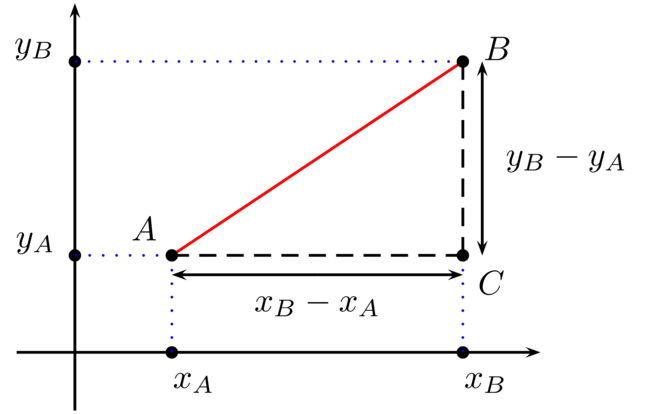
\includegraphics{Picture_FIGLabelFigPythagoreeBqLDUPICTPythagoreeBqLDU-for_eps.pdf}

%The result is on figure \ref{LabelFigPythagoreeBqLDU}.
%\newcommand{\CaptionFigPythagoreeBqLDU}{<+Type your caption here+>}
%\input{Fig_PythagoreeBqLDU.pstricks}

\end{multicols}
    \end{Aretenir}

\begin{proof}
    Nous allons utiliser le théorème de Pythagore. Pour cela nous construisons le triangle rectangle construit sur les points \( A\) et \( B\) comme indiqué sur le dessin. Le point \( C\) est le point de même abscisse que \( B\) et de même ordonnée que \( A\), c'est à dire que \( C\) est le point
    \begin{equation}
        C=(B_x,A_y).
    \end{equation}
    La droite \( AC\) est parallèle à l'axe des abscisses et la droite \( BC\) est parallèle à l'axe des ordonnées; elles sont donc perpendiculaires et le triangle \( ABC\) est un triangle rectangle en \( C\). Le théorème de Pythagore s'applique :
    \begin{equation}    \label{EqjLjEKr}
        \| AB \|=\sqrt{\| AC \|^2+\| BC \|^2}.
    \end{equation}
    Il reste à déterminer les longueurs \( \| AC \|\) et \( \| BC \|\). Le segment \( [AC]\) est horizontal et s'étend de l'abscisse \( A_x\) à l'abscisse \( B_x\), donc il est de longueur soit \( A_x-B_x\) soit \( B_x-A_x\), mais dans les deux cas nous avons
    \begin{equation}
        \| AC \|^2=(B_x-A_x)^2.
    \end{equation}
    De la même façon nous avons 
    \begin{equation}
        \| BC \|^2=(B_y-A_y)^2.
    \end{equation}
    En remplaçant dans \eqref{EqjLjEKr}, nous obtenons le résultat annoncé.
\end{proof}

%+++++++++++++++++++++++++++++++++++++++++++++++++++++++++++++++++++++++++++++++++++++++++++++++++++++++++++++++++++++++++++
\section{Exercices de géométrie repérée}
%+++++++++++++++++++++++++++++++++++++++++++++++++++++++++++++++++++++++++++++++++++++++++++++++++++++++++++++++++++++++++++

%---------------------------------------------------------------------------------------------------------------------------
\subsection{Géométrie brute}
%---------------------------------------------------------------------------------------------------------------------------


\Exo{Seconde-0045}

%---------------------------------------------------------------------------------------------------------------------------
\subsection{Placer et lire des coordonnées dans un repère}
%---------------------------------------------------------------------------------------------------------------------------

\Exo{Seconde-0001}
\Exo{Seconde-0002}
\Exo{Seconde-0007}

%---------------------------------------------------------------------------------------------------------------------------
\subsection{Milieu de segments}
%---------------------------------------------------------------------------------------------------------------------------

\Exo{Seconde-0056}
\Exo{Seconde-0012}
\Exo{Seconde-0055}
\Exo{Seconde-0011}

%---------------------------------------------------------------------------------------------------------------------------
\subsection{Longueur de segments}
%---------------------------------------------------------------------------------------------------------------------------

\Exo{Seconde-0008}
\Exo{Seconde-0003}
\Exo{Seconde-0004}
\Exo{Seconde-0005}
\Exo{Seconde-0006}
\Exo{Seconde-0009}
\Exo{Seconde-0010}
\Exo{Seconde-0013}
\Exo{Seconde-0021}
\Exo{Seconde-0019}
\Exo{Seconde-0020}

